\documentclass[12pt]{article}
\usepackage[utf8]{inputenc}
\usepackage[english]{babel}
\usepackage{graphicx}
\usepackage{algorithm}
\usepackage{algpseudocode}
\usepackage{hyperref}
\usepackage{listings}

\begin{document}

\begin{titlepage}
    \centering
	\Huge Artificial Nose\par
	\vspace{1cm}
	\Large Real-Time Systems, Embedded Computing Systems\par
	\vspace{1.5cm}
    \Large Luca Belluardo e Andrea Stevanato\par
    \vspace{1cm}
    \large a.stevanato.1995@gmail.com, luca.bellu95@gmail.com\par
    \large 
	\vfill
	{\large \today\par}
\end{titlepage}

\section{Introduction}
In this project a real-time application is developed to recognize smells from an
artificial nose. The sensor used for the application is an air quality gas 
sensor. The application is divided into five periodic tasks. Each task handles
a specific functionality of our application.

For the recognizing the image a neural network was trained. For what concerns
the neural network the Tensorflow framework was used.

The smells for which the neural network has been trained are: orange, coffee
and mustard. The final test accuracy of the neural network is about $93\%$.

\section{The tasks}
In our application we have 5 periodic tasks (Figure \ref{tdiagram}): graphic
task, sensor task, neural network task (made with Tensorflow), keyboard task
and the store image task.

The main function sets everything up for the tasks, except for the store
image task. The keyboard task is in charge to activate the store image task
when the \texttt{ENTER} key is pressed. If the store image task is already in
execution and the \texttt{ENTER} key is pressed this it's terminated.
Before start the store image task it's possible to write the name of the
directory in which the images will be saved; if no name it's writed the
images will be saved into \textit{image\_neural\_network} directory.

The sensor is read by an Arduino M0 pro; the sampled data read by arduino
are sent via the serial port to our application and read by the sensor
task. All the tasks are terminated by the main when the user presses the
\texttt{ESC} key.

\begin{figure}[H]
    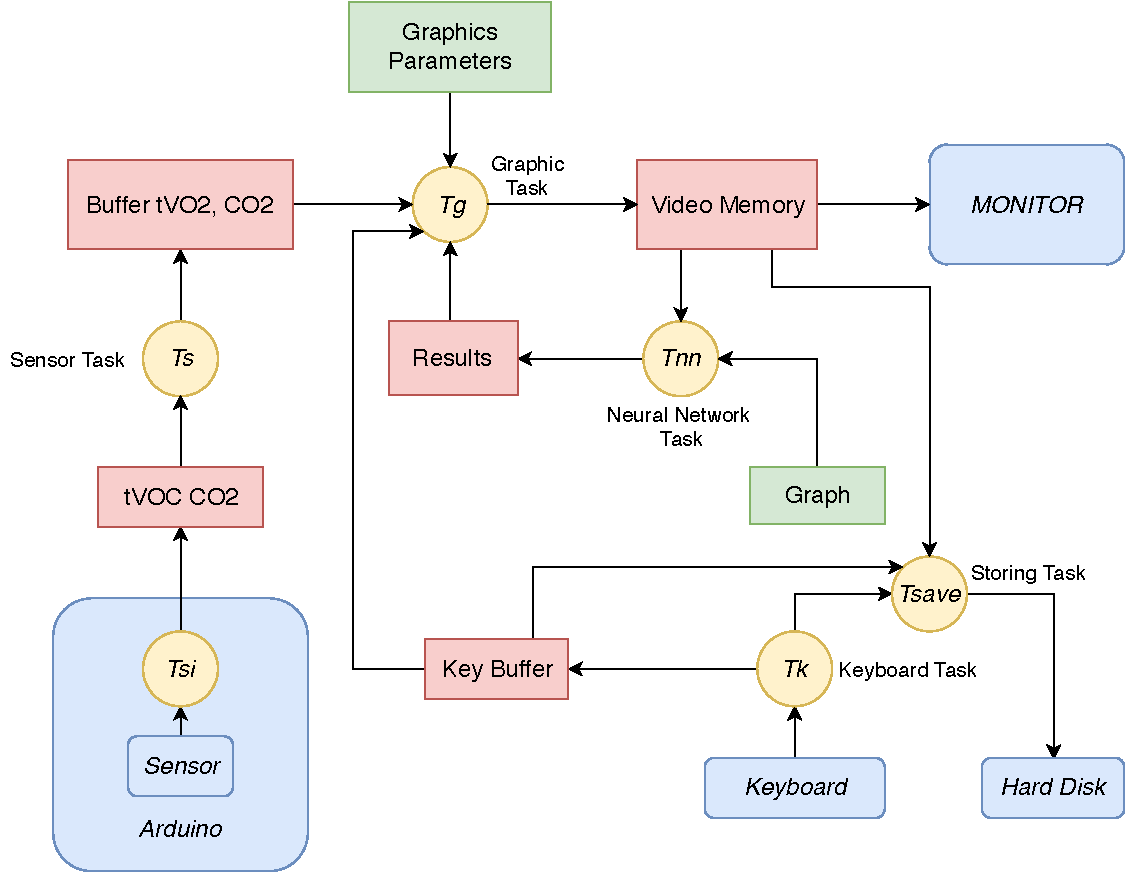
\includegraphics[width=\textwidth]{diagram.pdf}
    \caption{Task diagram}
    \label{tdiagram}
\end{figure}

\subsection{Main function}
In the main function [\ref{main}] all the tasks, except the store image task,
are started and the mutexes initialized. The mutexes are four, one for the
buffer that contains the values read from the sensor, one for the results
given by the neural network, one to update the deadline miss and WCET values
in the task table and one for the buffer that contains the keyboard input. The
main also starts allegro and waits for the termination of the keyboard task.
Once the keyboard task terminates the main cancels all other task and wait
for their termination.

\begin{algorithm}[H]
\caption{Main}
\label{main}

\begin{algorithmic}
\State $T\gets$ \textit{tasks to be started}
\State Mutexes and allegro initialization
\For{$t \in T$}
    \State start $t$
\EndFor

\Repeat
\Until{\textit{wait for termination of keyboard task}}

\For{$t \in T$} 
    \State cancel and join $t$
\EndFor

\end{algorithmic}
\end{algorithm}

\subsection{Graphic Task}

The graphic task [\ref{graphic}] prints the interface (Figure
\ref{interface}) of our application. The interface is divided into different
areas which contains for each one: the graph, the image, the results, the
legend, the current values, the information about tasks and the current
mode (\texttt{SAVING} or \texttt{WRITING}) followed by, if present, the
keyboard input.

\begin{figure}[H]
    \centering
    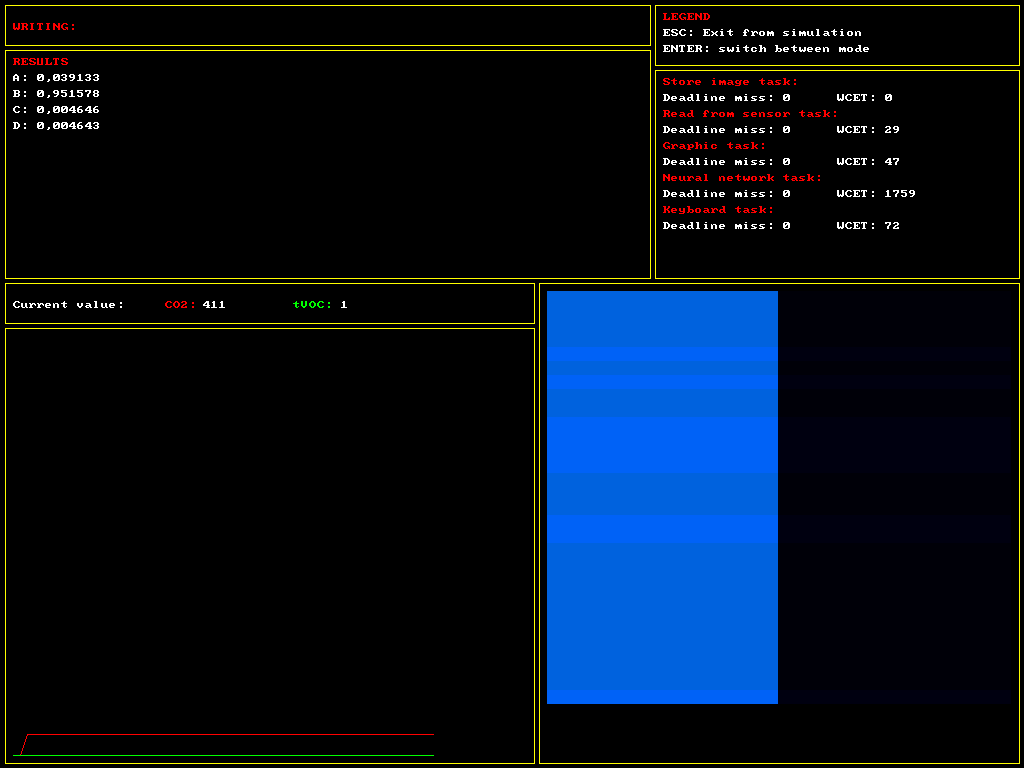
\includegraphics[width=0.75\textwidth]{images/interface.png}
    \caption{Interface of application}
    \label{interface}
\end{figure}

\begin{algorithm}[H]
\caption{Graphic task}
\label{graphic}

\begin{algorithmic}
\State $p\gets$ \textit{task period}
\State set activation task
\State draw interface background

\Loop
\State draw graph and image
\State draw results given by neural network
\State draw current values read from sensor
\State draw keyboard input
\State draw task information
\State wait for next activation
\EndLoop

\end{algorithmic}
\end{algorithm}

\subsubsection*{Graph}
The graph (Figure \ref{graph}) is made with the values sampled from the 
sensor. These values are plotted with two different colors: red for the $CO2$
and green for the $tVOC$. The graph contains at most $N$ readings of both values.

\begin{figure}[H]
    \centering
    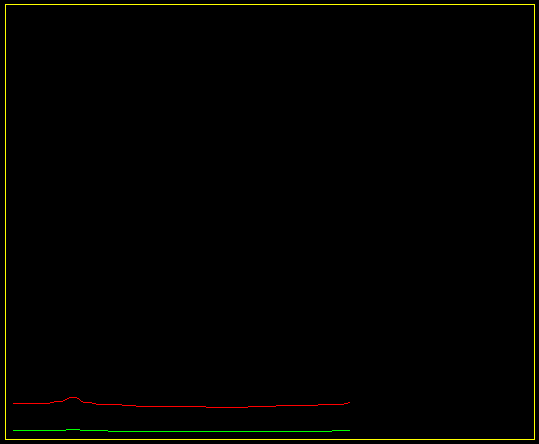
\includegraphics[scale=0.55]{images/graph.png}
    \caption{Graph }
    \label{graph}
\end{figure}

\subsubsection*{Image}
The image (Figure \ref{image}) is made with the last $N$ values sampled from
the sensor. The allegro color mode is set to 15-bit. In the 15-bit mode each
color is represented by 5-bit.

The sensor samples two data, the CO2 and the tVOC. Each value is a 15-bit
number and so we represent the values read as colors in 15-bit. The image is
divided in two parts, left and right. In the left side we draw the CO2 and in
the right the tVOC. Even if each value could be potentially from $0$ to
$2^{16} - 1$ the CO2 value is between $400$ and $8192$ and the tVOC value is
between $0$ and $1187$. These infomations are taken from the datasheet of
sensor.

Whenever a new pair of values are read from the sensor, the image is moved
one line below, removing one line at the bottom of the image and adding the
new line, which contains the new values, on the top of the image.

\begin{figure}[H]
    \centering
    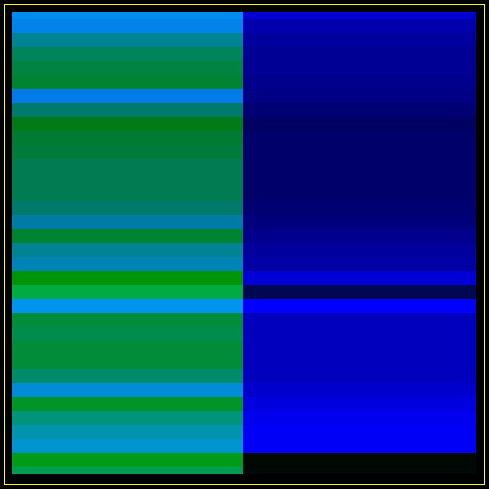
\includegraphics[scale=0.60]{images/image.png}
    \caption{Image}
    \label{image}
\end{figure}

\subsubsection*{Results}
This area shows the results (Figure \ref{results}) of neural network having
the current image as input. The lines represent the classes for which the
neural network was trained and the values are the neural network output.

\begin{figure}[H]
    \centering
    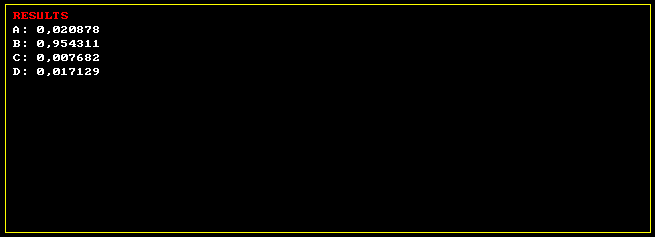
\includegraphics[width=\textwidth]{images/results.png}
    \caption{Result}
    \label{results}
\end{figure}

\subsubsection*{Current values}
This area shows the current values (Figure \ref{values}) sampled from the sensor.

\begin{figure}[H]
    \centering
    
\includegraphics[width=\textwidth]{images/values.png}
    \caption{Current values}
    \label{values}
\end{figure}

\subsubsection*{Task information}
This area (Figure \ref{task_info}) contains the information about deadline
misses and WCET for each task of our application. Before a task suspend it self
waiting for the next activation, it updates its values in the task table.

\begin{figure}[H]
    \centering
    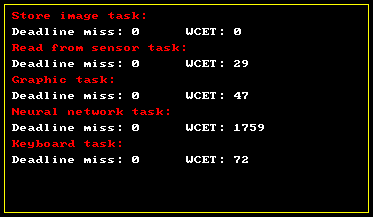
\includegraphics[scale=0.75]{images/task_info.png}
    \caption{Task information}
    \label{task_info}
\end{figure}

\subsubsection*{Current status}
This area (Figure \ref{save_write}) gives the information about the current
mode, printed on the left side; on the right side there is the name of the
directory in which the image are saved.

\begin{figure}[H]
    \centering
    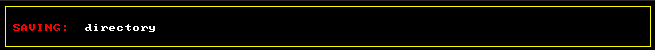
\includegraphics[scale=0.75]{images/saving.png}
    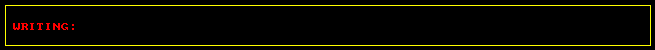
\includegraphics[scale=0.75]{images/writing.png}
    \caption{Saving and writing mode}
    \label{save_write}
\end{figure}

\subsection{Sensor task}
The sensor task [\ref{sensortask}] reads the values from the arduino which
sends on serial port the values taken from the sensor. The read values are
stored into an array and used by the graphic task to draw the image and the
graph; the current read values are also standalone printed by the graphic
task.

\begin{algorithm}[H]
\caption{Sensor task}
\label{sensortask}

\begin{algorithmic}
\State $p\gets$ \textit{task period}
\State initialization $data\_q$
\State initialization serial port
\State set activation task

\Loop
\State $data\_q\gets data\_q$ + values read from sensor
\State wait for next activation
\EndLoop

\end{algorithmic}
\end{algorithm}

\subsection{Neural network task}
The neural network task [\ref{nntask}] recognizes the smells using as input the
current image created with the values sampled by the sensor.

\begin{algorithm}[H]
\caption{Neural network task}
\label{nntask}

\begin{algorithmic}
\State $p\gets$ \textit{task period}
\State Tensorflow initialization
\State set activation task

\Loop
\State $image\gets$ current image
\State $results\gets$ use neural network with given $image$
\State wait for next activation
\EndLoop

\end{algorithmic}
\end{algorithm}

\subsection{Keyboard task}
The keyboard task [\ref{ktask}] takes input from keyboard and puts it into
\textit{keyboard buffer}. The keyboard buffer is printed by the graphic task
in its area of interface. The string contained into keyboard buffer is the
directory, under \textit{image\_neural\_network}, where the images are saved
by the store image task. The keyboard task can be in two different mode:
\texttt{WRITING} or \texttt{SAVING}. The task is started in \texttt{WRITING}
mode. During this mode it's possible to write the name of the directory in
which the images are saved. The name can contain letters, numbers, minus,
underscore and point; it's also possible to delete the written characters
pressing the \texttt{BACKSPACE} key. Pressing the \texttt{ENTER} key, the
current mode is switched from the \texttt{WRITING} to the \texttt{SAVING}
mode or vice versa. When the \texttt{ESC} key is pressed the keyboard task
terminates causing the closing of our application.

\begin{algorithm}[H]
\caption{Keyboard task}
\label{ktask}

\begin{algorithmic}
\State $p\gets$ \textit{task period}
\State $cur\_mode\gets$ \texttt{WRITING}
\State create \textit{key\_buffer}
\State keyboard initialization
\State set activation task

\Repeat
\State $key\_pressed\gets$ key code from keyboard
\If {$key\_pressed$ == \texttt{ENTER}}
    \If {$cur\_mode$ == \texttt{WRITING}}
    \State $cur\_mode\gets$ \texttt{SAVING}
    \State start store image task
    \Else
    \State $cur\_mode\gets$ \texttt{WRITING}
    \State stop store image task and clean key\_buffer
    \EndIf
\ElsIf {$cur\_mode$ == \texttt{WRITING}}
    \If {$key\_pressed$ equal to letter, number, minus or point \textbf{and} \textit{key\_buffer} not full}
        \State \textit{key\_buffer} $\gets$ \textit{key\_buffer} + $key\_pressed$ 
    \ElsIf {\textit{key\_buffer} == \texttt{BACKSPACE} \textbf{and} \textit{key\_buffer} not empty}
        \State remove last element from \textit{key\_buffer}
    \EndIf
\EndIf

\Until {$key\_pressed$ != \texttt{ESC}}

\end{algorithmic}
\end{algorithm}

\subsection{Store image task}
The store image task [\ref{sitask}] is activated/terminated by keyboard task
when the \texttt{ENTER} key is pressed. Once the task is activated the image
are saved every $300$ milliseconds. The images saved by this task are used to
train the neural network for the recognizing of smells.

\begin{algorithm}[H]
\caption{Store image task}
\label{sitask}

\begin{algorithmic}
\State $p\gets$ \textit{task period}
\State $dir\gets$ \textit{path to directory where images are saved}
\State set activation task

\Loop
\State save image to $dir$
\State wait for next activation
\EndLoop

\end{algorithmic}
\end{algorithm}

\subsection{Scheduling}
In our application a task table (Listing \ref{ttable}) was created containing
all the task that have to be started by the main function. The parameters
that characterize a task are respectively: thread identifier, function to be
execute, priority, period, number of deadline miss and the WCET. At the
beginning the thread identifier is set to $-1$, once the task is activated
the thread identifier is updated. In case of deadline misses the application
increments the corresponding value on the task table. The real time
scheduling algorithm chosen is \texttt{SCHED\_FIFO}. The deadline corresponds
with the period.

\begin{lstlisting}[caption={Task table}, captionpos=b, label={ttable}]
Task task_table[] = {
    {-1, store_image_task, 20, 1000, 0, 0},
    {-1, read_from_sensor_task, 30, 500, 0, 0},
    {-1, graphic_task, 30, 100, 0, 0},
    {-1, neural_network_task, 25, 2000, 0, 0},
    {-1, keyboard_task, 30, 100, 0, 0}
};
\end{lstlisting}

\section{Neural network}
Regarding the neural network we used Tensorflow, an open-source software 
library for dataflow programming across a range of tasks. 

For training the neural network was used a python script
\href{https://www.tensorflow.org/hub/tutorials/image\_retraining}{retrain}
provided by Tensorflow. The retrain script use the Inception V3 architecture.
In this file a lot of configurations are possible. In our application we use
the default configurations and choose only the number of training steps.

The output of the retrain script is saved into a file that we have called
\texttt{graph.pb}. When the neural network task is activated, it loads this
file that is used by tensorflow for recognizing the image. Each pixel of
image is divided into three elements, one for each color: red, green and
blue; the value of each color for each pixel is stored into a third order
tensor, which is the input for the neural network.

\section{Results}

The first experiment was made with wine, vinegar, ethyl alcohol and perfume.
Using this smells the sensor goes into saturation and it is not able to
discriminate between the smells. The same results was achieved increasing the
distance between the smells and the sensor without no positive results.

After the first experiment the neural network was trained for recognizing
smells of orange, coffee and mustard. These smells was chosen due to their
limited CO2 and tVOC values. With these values we obtained good results. Once
the smell has been exposed to the sensor, it take some time to settle on a
value.

\end{document}